% 附录 R：尘埃等离子体：从刻蚀腔到等离子体晶体（v1.15.0 新增）
% 数值唯一来源：tmp/appR_calc.py -> tmp/appR_calc.txt（正文与门禁的唯一来源）
% 时间单位写成 yr/day，避免中文字符进入数学字体；全部数字可用仓库脚本复算。
% 版权口径：只借鉴经典教材与文献的物理结论、公式形式与题型；文字、数值与表格自拟并独立复算。
% 离线环境无法核验 DOI，故只给书名、作者、年份、卷期页。

\section{尘埃等离子体：多出来的第三个尺度}
\label{sec:app-r-scale}

前面所有章节的等离子体只有两种带电成分：电子与离子。一旦里面出现微米级的固体颗粒（尘埃，dust），
系统的"自由度数"就变了：颗粒半径 $a\sim0.01$--$10\ \mathrm{\mu m}$、间距 $\Delta$ 从几十
$\mathrm{\mu m}$ 到几十 m（由尘埃密度决定）、每个颗粒带 $10$--$10^{5}$ 个电子电荷，而质量却是
同一等离子体里离子的 $10^{5}$--$10^{14}$ 倍（以 $a=0.01$--$10\ \mathrm{\mu m}$、$\rho\approx2000\
\mathrm{kg/m^3}$ 对氩离子估算；本附录四个工况落在 $5\times10^{9}$--$10^{13}$）。带电重、比荷极小、又能被相机直接拍到——这三条让尘埃等离子体（dusty /
complex plasma）成为唯一能"看见"单个粒子运动的等离子体。本附录的四个工况里，电子密度跨十三个数量级、
德拜长度跨六个数量级：

\begin{table}[htbp]
  \centering
  \caption{本附录的四个工况。$T_e$ 单位 eV，$n_e$、$n_d$ 单位 $\mathrm{m^{-3}}$，$a$ 单位
    $\mathrm{\mu m}$，$\rho$ 单位 $\mathrm{kg/m^3}$，$T_d$ 单位 eV（尘埃动能温度）。}
  \label{tab:app-r-map}
  \begin{tabular}{@{}p{2.4cm}p{0.9cm}p{1.1cm}p{1.9cm}p{1.1cm}p{1.3cm}p{1.7cm}p{1.1cm}@{}}
    \toprule
    工况 & 气体 & $T_e$ & $n_e$ & $a$ & $\rho$ & $n_d$ & $T_d$ \\
    \midrule
    C1 刻蚀工艺腔 & Ar & $3$ & $1\times10^{17}$ & $0.5$ & $2000$ & $1\times10^{12}$ & $0.0259$ \\
    C2 实验室尘埃晶体 & Ar & $3$ & $1\times10^{15}$ & $4.8$ & $1510$ & $1\times10^{9}$ & $0.03$ \\
    C3 聚变边界 & D & $15$ & $2\times10^{19}$ & $1.0$ & $2000$ & $1\times10^{10}$ & --- \\
    C4 星际介质 & H & $1$ & $1\times10^{6}$ & $0.1$ & $2000$ & $1\times10^{-6}$ & --- \\
    \bottomrule
  \end{tabular}
\end{table}

判断一个尘埃问题难不难，只需要三个无量纲数：$a/\lambda_D$ 决定用哪套充电理论，$t_{\mathrm{charge}}/T$
决定颗粒跟不跟得上驱动，$\Gamma$ 决定这堆颗粒是气体还是晶体。本附录按这三个数依次展开。
德拜长度沿用附录 Q 的工程式 \eqref{eq:app-q-debye}，四个工况分别给出
$40.72$、$407.17$、$6.44\ \mathrm{\mu m}$ 与 $7.43\ \mathrm{m}$——同一条公式跨了六个量级，
这就是为什么"尘埃等离子体"这个名字下面藏着完全不同的物理。

\textbf{出处：} Shukla \& Mamun《Introduction to Dusty Plasma Physics》（IoP, 2002）第 1--2 章的
课题地图与参数范围；Fortov \& Morfill《Complex and Dusty Plasmas: From Laboratory to Space》
（CRC Press, 2010）第 1 章；本书附录 Q 式 \eqref{eq:app-q-debye}（德拜长度）与附录 P 表 P.1
（低温工况）；第 2 章补充材料（耦合参数 $\Gamma$ 的一般定义）。

\begin{figure}[htbp]
\centering
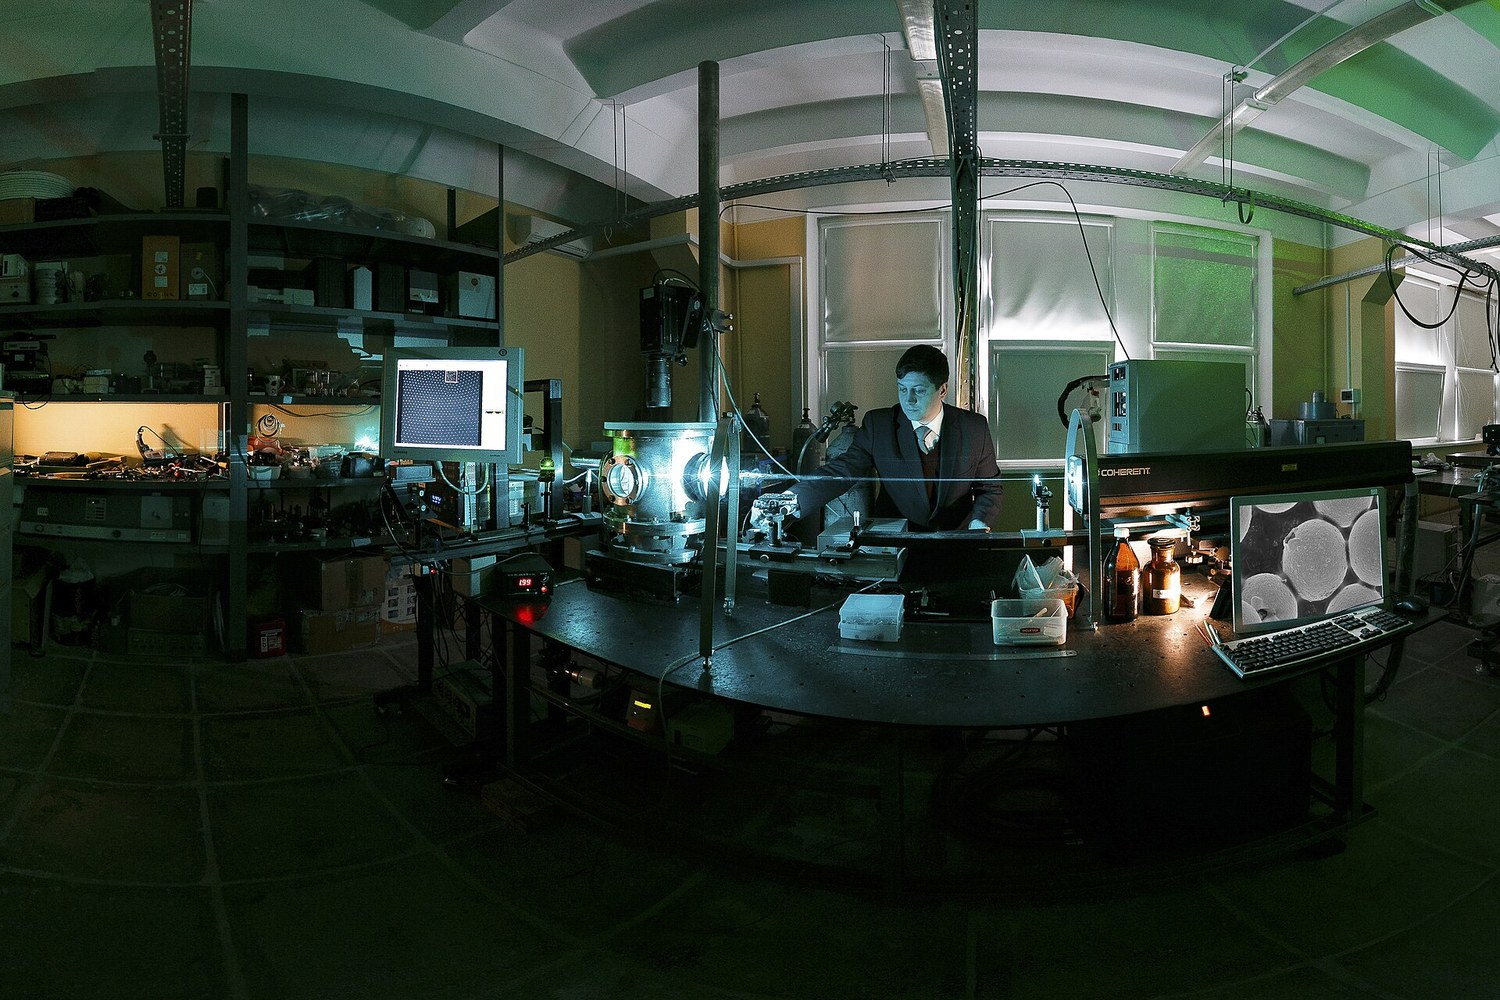
\includegraphics[width=0.78\textwidth]{../figures/dust_plasma_lab.jpg}
\caption{尘埃等离子体诊断实验台：多出来的第三个尺度。尘埃颗粒比离子重十到十二个数量级、带电上万电子，却能被等离子体托住并排成晶体——本节讨论的 OML 充电、强耦合与 Havnes 参数，都能在这样的实验台上逐项测出来。}
\label{fig:photo-appr}
\figsource{Stanislav Liubauskas，CC BY 4.0（Wikimedia Commons）}
\end{figure}

\section{尘埃怎么带电：OML 电流平衡}
\label{sec:app-r-charge}

颗粒插进等离子体后，电子跑得快、先撞上去，颗粒带负电，直到两种电流相等。在
$a/\lambda_D\ll1$、无强磁场、无二次电子与光电发射的条件下，用轨道运动限制（OML）写法：

\begin{equation}
  I_e = -\pi a^2 e n_e v_{th,e}\exp\!\left(\frac{e\phi_d}{k_{\!B}T_e}\right),
  \qquad
  I_i = \pi a^2 e n_i v_{th,i}\left(1-\frac{e\phi_d}{k_{\!B}T_i}\right),
  \qquad
  I_e + I_i = 0,
  \label{eq:app-r-oml}
\end{equation}

其中 $v_{th,s}=\sqrt{8k_{\!B}T_s/(\pi m_s)}$，$\phi_d<0$ 是颗粒相对等离子体的电位。取
$n_i=n_e$、$z=e|\phi_d|/(k_{\!B}T_e)$、$\tau=T_i/T_e$，平衡条件约掉全部几何因子与密度：

\begin{equation}
  \ee^{z} = \frac{1}{1+z/\tau}\sqrt{\frac{m_i}{\tau m_e}}.
  \label{eq:app-r-z}
\end{equation}

式 \eqref{eq:app-r-z} 只含温度比与质量比，所以\textbf{颗粒电位与半径、与密度都无关}：对氩气
（$T_i=300\ \mathrm{K}$、$T_e=3\ \mathrm{eV}$，$\tau=0.0086$）解得 $z=2.359$，
$\phi_d=7.077\ \mathrm{V}$。电荷则由半径决定：

\begin{equation}
  Z_d = \frac{4\pi\eps_0 a\phi_d}{e},
  \qquad
  Z_d \approx 1.638\times10^{3}\left(\frac{a}{\mathrm{\mu m}}\right)
  \left(\frac{T_e}{\mathrm{eV}}\right)
  \quad\text{(Ar, }T_i=300\ \mathrm{K}\text{，取 }z\approx2.36\text{ 为常数)}.
  \label{eq:app-r-zd}
\end{equation}

\begin{table}[htbp]
  \centering
  \caption{四个工况的充电结果。$\lambda_D$ 单位 $\mathrm{\mu m}$（C4 为 m），
    $Z_d$ 以电子电荷为单位。}
  \label{tab:app-r-charge}
  \begin{tabular}{@{}p{1.6cm}p{2.4cm}p{2.2cm}p{1.2cm}p{1.6cm}p{2.0cm}p{2.2cm}p{2.2cm}@{}}
    \toprule
    工况 & $\lambda_D$ & $a/\lambda_D$ & $z$ & $\phi_d$ [V] & $Z_d$ & $Q_d$ [C] & $t_{\mathrm{charge}}$ \\
    \midrule
    C1 & $40.72$ & $0.0123$ & $2.359$ & $7.077$ & $2.46\times10^{3}$ & $3.94\times10^{-16}$ & $27.0\ \mathrm{ns}$ \\
    C2 & $407.17$ & $0.0118$ & $2.359$ & $7.077$ & $2.36\times10^{4}$ & $3.78\times10^{-15}$ & $281.2\ \mathrm{ns}$ \\
    C3 & $6.44$ & $0.1553$ & $2.776$ & $41.63$ & $2.89\times10^{4}$ & $4.63\times10^{-15}$ & $0.178\ \mathrm{ns}$ \\
    C4 & $7.43\times10^{6}$ & $1.3\times10^{-8}$ & $1.195$ & $1.195$ & $83.0$ & $1.33\times10^{-17}$ & $3.95\times10^{3}\ \mathrm{s}$ \\
    \bottomrule
  \end{tabular}
\end{table}

式 \eqref{eq:app-r-zd} 的用途是"心算"：半径 $1\ \mathrm{\mu m}$ 的颗粒在 $3\ \mathrm{eV}$ 氩气里带
约 $5\times10^{3}$ 个电荷；要带 $10^{5}$ 个电荷，半径得做到 $20\ \mathrm{\mu m}$，或把电子温度提到
$60\ \mathrm{eV}$。注意 $z$ 与密度无关这件事的边界：它来自 $n_i=n_e$ 的假设，一旦尘埃多到把
电子吃掉（第 R.5 节），准中性条件变成 $n_i=n_e+n_dZ_d$，$z$ 就开始随密度变。

\begin{tip}{OML 的适用边界：四个前提逐条查}{tip-appr-limit}
式 \eqref{eq:app-r-oml} 的第一行有三个前提，缺一个就换理论：\textbf{（1）几何}
$a/\lambda_D\lesssim0.1$——本附录 C1、C2 满足，C3 的 $0.155$ 已在边缘，颗粒大到与德拜尺度可比时
必须用径向运动（ABR）类理论（见附录 Q 第 Q.2 节）；\textbf{（2）温度}离子不能真的取 $0$：
$\tau\to0$ 时式 \eqref{eq:app-r-oml} 的离子电流发散，应改用玻姆通量形式的离子电流，本附录取中性
气体温度 $300\ \mathrm{K}$（$\tau\approx0.009$）的正规写法；\textbf{（3）发射}强电子发射
（二次电子、光电发射、热电子）会让颗粒电位反号甚至变成正的，空间环境正是这种情况（第 R.9 节）；
\textbf{（4）磁场}磁化时电子沿磁力线收集，收集截面变成各向异性。
\end{tip}

\textbf{出处：} OML 收集理论的原始表述见 Mott-Smith \& Langmuir, \emph{Physical Review}
\textbf{28}, 727--763 (1926)（附录 Q 已引）；尘埃充电的电流平衡写法与 $z\approx2.4$ 的量级见
Shukla \& Mamun (2002) 第 2 章；Fortov 等, \emph{Physics Reports} \textbf{421}, 1--103 (2005)
第 3 节（OML 的适用边界与失效机制）；本书附录 Q 第 Q.2 节（收集理论的几何判据）。

\section{充电要多久：颗粒跟不跟得上射频}
\label{sec:app-r-time}

带电快慢由"电子热流"决定，用平衡电荷除以未带电时的电子电流做量级估计：

\begin{equation}
  t_{\mathrm{charge}} = \frac{Q_d}{I_{e0}},
  \qquad
  I_{e0} = \pi a^2 e n_e v_{th,e}
  = \pi a^2 e n_e\sqrt{\frac{8k_{\!B}T_e}{\pi m_e}}.
  \label{eq:app-r-tcharge}
\end{equation}

与式 \eqref{eq:app-r-zd} 不同，充电时间\textbf{强依赖密度}：C1 的 $I_{e0}=1.46\times10^{-8}\ \mathrm{A}$
给出 $t_{\mathrm{charge}}=27.0\ \mathrm{ns}$，C2 是 $281.2\ \mathrm{ns}$，C3 只要
$0.178\ \mathrm{ns}$，而 C4（星际，$n_e=10^{6}\ \mathrm{m^{-3}}$）要 $3.95\times10^{3}\ \mathrm{s}$
——将近 $66$ 分钟。把这个时间与驱动周期比：

\begin{itemize}
  \item $13.56\ \mathrm{MHz}$ 射频（周期 $73.75\ \mathrm{ns}$）：C1 的 $t_{\mathrm{charge}}/T=0.366<1$，
        颗粒在\textbf{一个射频周期内}就充到准平衡，因此可以用"平衡电荷"做静力学分析；但瞬时鞘层
        电位仍在周期内变化，颗粒电荷跟着抖，这是射频鞘能"推"颗粒的根源；
  \item 附录 P 的 $10\ \mathrm{kHz}$ 大气压 DBD（周期 $100\ \mathrm{\mu s}$）：
        $t_{\mathrm{charge}}/T=2.7\times10^{-4}$，充电远远快于驱动变化，颗粒始终跟着瞬时电位；
  \item 反过来，C4 的 $66\ \mathrm{min}$ 意味着星际尘埃的电荷是\textbf{光照与碰撞历史的平均值}，
        不能用瞬时平衡去算它的轨道演化。
\end{itemize}

\textbf{出处：} 充电时间的标度与射频等离子体中的颗粒行为见 Fortov 等, \emph{Physics Reports}
\textbf{421}, 1--103 (2005) 第 4 节；Bouchoule《Dusty Plasmas: Physics, Chemistry and
Technological Impacts in Plasma Processing》（Wiley, 1999）第 3 章；附录 P 表 P.1（$10\ \mathrm{kHz}$
DBD 工况）；本书第 11 章（鞘层的时间响应）。

\section{强耦合与晶体：$\Gamma$ 的两种定义}
\label{sec:app-r-crystal}

尘埃之间是库仑排斥，颗粒的"温度" $T_d$ 由速度涨落定义，于是可以照搬第 2 章补充材料的耦合参数，
只是把电荷换成 $Q_d$、把 Wigner--Seitz 半径换成颗粒间距：

\begin{equation}
  \Delta = \left(\frac{3}{4\pi n_d}\right)^{1/3},
  \qquad
  \Gamma = \frac{Q_d^{2}}{4\pi\eps_0\Delta k_{\!B}T_d}
  = \frac{Z_d^2\,(1.44\ \mathrm{eV\cdot nm})}{\Delta\,[\mathrm{nm}]\,k_{\!B}T_d\,[\mathrm{eV}]}.
  \label{eq:app-r-gamma}
\end{equation}

这里有一个必须讲清楚的\textbf{定义陷阱}：把分母里的距离换成颗粒半径 $a$（有的作者用接触距离 $2a$），
同一个实验就会算出两个不同的 $\Gamma$。本附录把这两种写法都列出来，因为它们的比值恰好是
$\Delta/a\approx124$--$130$——引用文献时不写明用哪个距离，数字就没法比较。更麻烦的是，尘埃等离子体
的屏蔽长度与间距可比（$\kappa=\Delta/\lambda_D\approx1.5$），必须用 Yukawa 修正：

\begin{equation}
  \Gamma_{\mathrm{eff}} = \Gamma\left(1+\kappa+\frac{\kappa^{2}}{2}\right)\ee^{-\kappa},
  \qquad
  \kappa = \frac{\Delta}{\lambda_D},
  \qquad
  \Gamma_{\mathrm{eff}}\gtrsim170 \;\Rightarrow\; \text{库仑晶体}.
  \label{eq:app-r-yukawa}
\end{equation}

\begin{table}[htbp]
  \centering
  \caption{耦合与屏蔽：同一个 $\Gamma$ 在两种距离定义下差两个数量级，Yukawa 修正则决定它是否还有效。
    $\Delta$ 单位 $\mathrm{\mu m}$（C4 为 m）。}
  \label{tab:app-r-gamma}
  \begin{tabular}{@{}p{2.1cm}p{1.9cm}p{1.8cm}p{1.8cm}p{1.3cm}p{1.6cm}p{1.9cm}p{2.3cm}@{}}
    \toprule
    工况 & $\Delta$ & $\Gamma(\Delta)$ & $\Gamma(a)$ & $\kappa$ & 屏蔽因子 & $\Gamma_{\mathrm{eff}}$ & 结论 \\
    \midrule
    C1 & $62.04$ & $5.41\times10^{3}$ & $6.71\times10^{5}$ & $1.524$ & $0.803$ & $4.35\times10^{3}$ & 强耦合 \\
    C2 & $620.35$ & $4.31\times10^{4}$ & $5.57\times10^{6}$ & $1.524$ & $0.803$ & $3.46\times10^{4}$ & 强耦合（晶体） \\
    C3 & $287.94$ & $4.18\times10^{3}$ & $1.20\times10^{6}$ & $44.73$ & $\sim10^{-17}$ & $1.6\times10^{-13}$ & 屏蔽切断 \\
    C4 & $62.04$ & $1.60\times10^{-5}$ & $9.92\times10^{3}$ & $8.345$ & $0.0105$ & $1.7\times10^{-7}$ & 弱耦合气体 \\
    \bottomrule
  \end{tabular}
\end{table}

表 \ref{tab:app-r-gamma} 的两行极端值是本节的结论：\textbf{C2 是晶体}（$\Gamma_{\mathrm{eff}}$
比熔化判据高两个数量级），\textbf{C3 不是}——聚变边界的德拜长度只有 $6.44\ \mathrm{\mu m}$，而颗粒
间距 $288\ \mathrm{\mu m}$，$\ee^{-44.7}$ 把相互作用彻底切断，尘埃在那里只是一群各自独立的重离子。
所以"聚变边界有没有尘埃晶体"这个问题的正确答案是：没有，而且原因可以写成一个数
$\kappa=44.7$。判据 $\Gamma_{\mathrm{eff}}\gtrsim170$ 来自单分量等离子体（OCP）的熔化线，
Yukawa 系统的熔化线随 $\kappa$ 平移，实验上观测尘埃晶体时报告的 $\Gamma_{\mathrm{eff}}$ 常在
$10^{4}$ 量级，比 $170$ 高得多——差异来自强耗散、有限粒子数与约束势，这也是"判据给量级、
不给结论"的又一个例子。

\textbf{出处：} Ichimaru, \emph{Reviews of Modern Physics} \textbf{54}(4), 1017--1059 (1982)
（OCP 熔化判据 $\Gamma_c\approx170$）；Hamaguchi, Farouki \& Dubin, \emph{Physical Review E}
\textbf{56}(4), 4671--4682 (1997)（Yukawa 系统相图与熔化线）；Thomas 等, \emph{Physical Review
Letters} \textbf{73}(5), 652--655 (1994) 与 Hayashi \& Tachibana, \emph{Japanese Journal of
Applied Physics} \textbf{33}, L804--L806 (1994)（尘埃晶体的实验观测）；本书第 2 章补充材料
（耦合参数 $\Gamma$ 与 Wigner--Seitz 半径）。

\section{Havnes 参数：尘埃什么时候把电子吃光}
\label{sec:app-r-havnes}

前面的计算都假设"尘埃只是示踪物，不改背景"。这个假设可以用一个数检查——Havnes 参数：

\begin{equation}
  P = \frac{n_d Z_d}{n_e},
  \qquad
  \lambda_{\mathrm{eff}} = \frac{\lambda_D}{\sqrt{1+P}}.
  \label{eq:app-r-havnes}
\end{equation}

$P$ 就是"被尘埃吸走的电子占自由电子的比例"：$P\ll1$ 时可以只算充电、不管背景；$P\gtrsim1$ 时
必须把尘埃密度与背景密度联立求解，屏蔽长度也被压短。

\begin{table}[htbp]
  \centering
  \caption{Havnes 参数与临界尘埃密度。$\lambda_D$、$\lambda_{\mathrm{eff}}$ 单位
    $\mathrm{\mu m}$（C4 为 m），$n_d(P=1)$ 单位 $\mathrm{m^{-3}}$。}
  \label{tab:app-r-havnes}
  \begin{tabular}{@{}p{2.6cm}p{1.8cm}p{1.9cm}p{1.9cm}p{2.6cm}p{3.2cm}@{}}
    \toprule
    工况 & $P$ & $\lambda_D$ & $\lambda_{\mathrm{eff}}$ & $n_d(P=1)$ & 判据 \\
    \midrule
    C1 & $0.0246$ & $40.72$ & $40.23$ & $4.07\times10^{13}$ & 现在安全，密度再高 $40$ 倍即失效 \\
    C2 & $0.0236$ & $407.17$ & $402.45$ & $4.24\times10^{10}$ & 现在安全，密度再高 $40$ 倍即失效 \\
    C3 & $1.45\times10^{-5}$ & $6.44$ & $6.44$ & $6.92\times10^{14}$ & 可忽略 \\
    C4 & $8.3\times10^{-11}$ & $7.43\times10^{6}$ & $7.43\times10^{6}$ & $1.2\times10^{4}$ & 完全可忽略 \\
    \bottomrule
  \end{tabular}
\end{table}

表 \ref{tab:app-r-havnes} 给出一条\textbf{工程警戒线}：刻蚀腔里尘埃密度达到
$4\times10^{13}\ \mathrm{m^{-3}}$（比本附录的假设高 $40$ 倍）时，"尘埃只是少量污染物"的图像就不成立，
颗粒会互相屏蔽并把等离子体电位抬高。反过来，C3、C4 的 $P$ 只有 $1.45\times10^{-5}$ 与
$8.3\times10^{-11}$，比 C1 小三个多与八个多数量级，
那两种环境里"尘埃不影响背景"是安全的。注意 $n_d(P=1)=n_e/Z_d$ 与 $Z_d\propto a$ 合起来意味着：
\textbf{颗粒越小，同样的质量能带走的电子越多}，所以纳米颗粒的临界数密度比微米颗粒高。

\textbf{出处：} Havnes, Morfill \& Goertz, \emph{Journal of Geophysical Research} \textbf{89},
10999--11003 (1984)（$P$ 参数与尘埃云电位的原始讨论）；Fortov \& Morfill (2010) 第 2 章
（$P\gtrsim1$ 时的联立求解与屏蔽缩短）；Shukla \& Mamun (2002) 第 3 章。

\section{尘埃声波：比离子声速慢五个量级}
\label{sec:app-r-wave}

尘埃等离子体里有一支"慢波"：恢复力来自电子与离子的压强，惯性全部由尘埃提供。在
$a\ll\lambda_D$、$\kappa\lesssim1$、弱耦合（$\Gamma_{\mathrm{eff}}$ 不大）的条件下，色散关系是
$\omega^{2}=k^{2}c_{DA}^{2}/(1+k^{2}\lambda_D^{2})$，长波极限给出尘埃声速：

\begin{equation}
  c_{DA} = \omega_{pd}\lambda_D
  = \sqrt{\frac{Z_d^{2}n_d k_{\!B}T_{\mathrm{eff}}}{n_e m_d}},
  \qquad
  T_{\mathrm{eff}} = \frac{T_eT_i}{T_e+T_i}
  \;\xrightarrow{\;T_i\ll T_e\;}\; T_i,
  \qquad
  \lambda = \frac{2\pi}{k}.
  \label{eq:app-r-cda}
\end{equation}

代入 C1：$c_{DA}=1.5455\ \mathrm{cm/s}$，而同工况的氩离子声速 $c_s=2691.8\ \mathrm{m/s}$——
比值 $1.74\times10^{5}$，整整五个数量级。这不是数学巧合，而是惯性的代价：尘埃质量是离子的
$1.6\times10^{10}$ 倍，$\omega_{pd}$ 也降到 $4.1\times10^{3}\ \mathrm{rad/s}$（C1）
与 $48\ \mathrm{rad/s}$（C2），而氩离子的 $\omega_{pi}=6.6\times10^{7}\ \mathrm{rad/s}$——低了四到六个量级。
慢的好处是"看得见"：

\begin{itemize}
  \item $\lambda=1\ \mathrm{mm}$ 时 $f=c_{DA}/\lambda=15.45\ \mathrm{Hz}$；$\lambda=10\ \mathrm{mm}$
        时 $1.55\ \mathrm{Hz}$。用一台每秒几百帧的相机就能拍到一个波峰走过标尺，相速度可以直接
        从两帧之间的位移读出——这在离子声波上是做不到的；
  \item C2 的 $c_{DA}=0.1815\ \mathrm{cm/s}$（$f=1.82\ \mathrm{Hz}$，$\lambda=1\ \mathrm{mm}$），
        比 C1 慢 $8.5$ 倍——因为 $c_{DA}\propto Z_d\sqrt{n_d/n_e}/\sqrt{m_d}$：C2 的电荷只多
        $9.6$ 倍，质量却大 $668$ 倍，惯性的代价盖过了电荷与密度的收益；
  \item C3 不能用这支波：$\kappa=44.7$（表 \ref{tab:app-r-gamma}），屏蔽把长波截断；强耦合的
        C2 还有另一支\textbf{尘埃晶格波}（相邻颗粒在约束势阱里的小振幅振荡），它的频率与
        $\omega_{pd}$ 同量级，但必须用声子语言描述。
\end{itemize}

\textbf{出处：} Rao, Shukla \& Yu, \emph{Planetary and Space Science} \textbf{38}(4), 543--546
(1990)（尘埃声波的原始色散关系）；Shukla \& Mamun (2002) 第 4 章（慢波家族与适用条件）；
Bouchoule (1999) 第 4--5 章（实验观测与晶格波）；本书第 4 章补充材料（离子声波的短波修正，
与本节的 $k\lambda_D$ 条件同源）。

\section{鞘层中的悬浮：重力与电场力谁赢}
\label{sec:app-r-levitate}

颗粒要停在鞘层里，必须有一个高度让它受到的电场力抵消重力（浮力与离子拖曳是次级项）：

\begin{equation}
  m_d g = Q_d E(z),
  \qquad
  m_d = \frac{4}{3}\pi a^{3}\rho,
  \qquad
  E_{\mathrm{need}} = \frac{m_d g}{Q_d}
  \propto \frac{\rho\,a^{2}}{\phi_d}.
  \label{eq:app-r-balance}
\end{equation}

把附录 P 的鞘层参数（$V_s=100\ \mathrm{V}$、$s=0.633\ \mathrm{mm}$）拿来当背景：平均场
$E_{\mathrm{mean}}=1.58\times10^{5}\ \mathrm{V/m}$，壁面处按 Child 律外推
$E_{\mathrm{wall}}=\tfrac{5}{3}E_{\mathrm{mean}}=2.63\times10^{5}\ \mathrm{V/m}$。四个工况需要的场是：

\begin{itemize}
  \item C1 的 $0.5\ \mathrm{\mu m}$ 尘：$E_{\mathrm{need}}=26.08\ \mathrm{V/m}$，只有
        $E_{\mathrm{mean}}$ 的 $1.65\times10^{-4}$；
  \item C2 的 $4.8\ \mathrm{\mu m}$ 尘：$E_{\mathrm{need}}=1815\ \mathrm{V/m}$，
        $E_{\mathrm{mean}}$ 的 $1.15\times10^{-2}$；
  \item C3（聚变边界）：$17.74\ \mathrm{V/m}$；C4（星际）：$6.18\ \mathrm{V/m}$。
\end{itemize}

结论不是"悬浮高度是多少"，而是\textbf{平衡点往哪边走}：鞘层电场从壁面的 $2.6\times10^{5}\ \mathrm{V/m}$
单调降到鞘边的 $0$，而需要的场只有 $10^{2}$--$10^{3}\ \mathrm{V/m}$，所以平衡点必然\textbf{紧贴鞘边}；
颗粒越大（或电荷越少），需要的场越高，平衡点就往鞘层内部、往电极方向移动。这正是射频刻蚀腔里
"颗粒聚在晶片上方、又被瞬时鞘层变化推进晶片表面"的力学原因。用纯 Child 律外推平衡位置只能给出
$x/s\sim10^{-6}$--$10^{-4}$ 这样的数，说明模型只可用于判方向：真实高度还要加预鞘、射频鞘与离子
拖曳的修正。另一条判据是颗粒\textbf{之间}的库仑力与重力之比（取间距 $\Delta$）：C1 为 $35.3$、
C2 为 $0.0486$——小颗粒由库仑力主导（会自己排成有序结构），大颗粒由重力主导（会往下掉）。

\textbf{出处：} Selwyn, Heidenreich \& Haller, \emph{Applied Physics Letters} \textbf{57}(18),
1876--1878 (1990)（射频等离子体中的颗粒陷阱与"尘埃云"观测）；Bouchoule (1999) 第 3 章
（悬浮力的量级比较）；本书第 11 章（鞘层与 Child--Langmuir 律）、附录 P 第 P.4 节
（$100\ \mathrm{V}$、$0.633\ \mathrm{mm}$ 鞘层）。

\section{从刻蚀腔到聚变堆：尘埃是缺陷与库存}
\label{sec:app-r-device}

同一个尘粒，在工艺腔里叫\textbf{缺陷源}，在聚变装置里叫\textbf{库存与安全问题}，两者的物理是同一
套公式：

\begin{itemize}
  \item \textbf{工艺侧}：颗粒落片一次就是一个致命缺陷（"杀手颗粒"），所以要算清它在鞘层里的
        平衡位置与运动时间尺度（第 R.3、R.7 节）。刻蚀腔的 $n_e=10^{17}\ \mathrm{m^{-3}}$、
        $T_e=3\ \mathrm{eV}$ 对应的 $t_{\mathrm{charge}}=27\ \mathrm{ns}$，颗粒一个射频周期内就充好电，
        因此\textbf{颗粒的输运是力学问题，不是充电问题}；附录 P 的工艺腔参数与颗粒污染讨论是同一背景；
  \item \textbf{聚变侧}：C3 的 $z=2.776$、$\phi_d=41.63\ \mathrm{V}$、$Z_d(1\ \mathrm{\mu m})
        =2.89\times10^{4}$、$t_{\mathrm{charge}}=0.178\ \mathrm{ns}$——充电极快，所以边界等离子体里的
        尘埃电荷始终取准平衡值；但 $\kappa=44.7$ 说明它们之间没有强耦合，尘埃是"独立的重离子"；
  \item \textbf{库存侧}：尘埃的比表面积 $3/(\rho a)=1500\ \mathrm{m^2/kg}$（$a=1\ \mathrm{\mu m}$、
        $\rho=2000\ \mathrm{kg/m^3}$），$100\ \mathrm{g}$ 尘埃就有 $150\ \mathrm{m^2}$ 内表面。
        若按氚面密度 $10^{21}\ \mathrm{m^{-2}}$ 估算，这些尘埃能吸附
        $1.5\times10^{23}$ 个氚原子，即 $0.751\ \mathrm{g}$ 氚——相当于附录 N 里
        $1.6$ 天的滞留产率（$0.460\ \mathrm{g/day}$）。
\end{itemize}

最后一条是本节想让读者记住的数量级判断：尘埃带来的氚库存\textbf{不大}（$0.75\ \mathrm{g}$，
即 $0.25\ \mathrm{mol}$），但它
\textbf{不受抽气系统控制}——它藏在固体里，只能靠诊断（附录 Q 的激光散射与光谱）与运行限制
（附录 N 的 $1\ \mathrm{kg}$ 库存窗口）一起管。

\textbf{出处：} Winter, \emph{Plasma Physics and Controlled Fusion} \textbf{40}(7), 1201--1212
(1998)（聚变装置中的尘埃）；Krasheninnikov, Smirnov \& Rudakov, \emph{Plasma Physics and
Controlled Fusion} \textbf{53}(8), 083001 (2011)（磁约束装置尘埃的来源、迁移与安全影响）；
本书附录 N（氚消耗 $46.0\ \mathrm{g/day}$、滞留 $0.460\ \mathrm{g/day}$、$1\ \mathrm{kg}$ 库存
$2170\ \mathrm{day}$ 触顶）与附录 P（工艺腔工况与颗粒污染）。

\section{空间与天体尘埃：光电充电与辐射压}
\label{sec:app-r-space}

空间环境里紫外线通量远大于等离子体热流，光电发射主导充电，颗粒电位\textbf{变成正的}：
$\phi_d=+1$--$+5\ \mathrm{V}$ 时，$a=0.1\ \mathrm{\mu m}$ 的颗粒带
$69.4$、$138.9$、$347.2$ 个正电荷。另一个决定尘埃命运的是辐射压与引力的比：

\begin{equation}
  \beta = \frac{F_{\mathrm{rad}}}{F_{\mathrm{grav}}}
  = \frac{3L}{16\pi cGM\rho a}
  = \frac{A}{\rho a},
  \qquad
  A = \frac{3L_\odot}{16\pi cGM_\odot}=5.742\times10^{-4}\ \mathrm{kg/m^2},
  \label{eq:app-r-beta}
\end{equation}

其中 $A$ 只依赖恒星参数，对太阳取上式数值。于是 $\beta$ 只由"$\rho a$"决定：$\rho=2000\ \mathrm{kg/m^3}$
时，$a=1\ \mathrm{\mu m}$ 的颗粒 $\beta=0.287$（被引力束缚，慢慢向里落）；$a=0.1\ \mathrm{\mu m}$ 的
颗粒 $\beta=2.87>1$（被辐射压吹出太阳系）；临界半径 $a_{\mathrm{crit}}=0.287\ \mathrm{\mu m}$。
这就是为什么行星际尘埃的尺度分布在小半径端有一个"悬崖"：$\beta$ 同时扮演筛子与加速器的角色。
最后对照 C4 的三个数：$t_{\mathrm{charge}}=3.95\times10^{3}\ \mathrm{s}$、$\Delta=62.04\ \mathrm{m}$、
$\Gamma(\Delta)=1.6\times10^{-5}$——星际尘埃是\textbf{弱耦合气体}，既不是晶体，也撑不起尘埃声波
（$\kappa=8.345$）。"尘埃等离子体"这个名字下面，耦合强度跨了八个数量级。

\textbf{出处：} Goertz, \emph{Reviews of Geophysics} \textbf{27}(2), 271--292 (1989)
（太阳系尘埃等离子体与光电充电）；Mendis \& Rosenberg, \emph{Annual Review of Astronomy and
Astrophysics} \textbf{32}, 419--463 (1994)（宇宙尘埃等离子体）；Whipple, \emph{Reports on
Progress in Physics} \textbf{44}(11), 1197--1250 (1981)（空间表面的电位）；本附录数值由
\texttt{appR\_calc.py} 独立复算。

\section{六道估算练习}
\label{sec:app-r-problems}

答案都可以用仓库脚本 \texttt{appR\_calc.py} 复算，量级对上即算通过。

\textbf{练习 1（充电电位与电荷）}。$T_e=3\ \mathrm{eV}$、$T_i=300\ \mathrm{K}$ 的氩气里有一颗
$a=4.8\ \mathrm{\mu m}$、$\rho=1510\ \mathrm{kg/m^3}$ 的颗粒。(1) 求 $\phi_d$ 与 $Z_d$；
(2) 换成 $a=0.1\ \mathrm{\mu m}$ 后 $\phi_d$ 变不变？

\textbf{解答}：由式 \eqref{eq:app-r-z} 解出 $z=2.359$，$\phi_d=2.359\times3=7.077\ \mathrm{V}$；
$Z_d=4\pi\eps_0a\phi_d/e=2.359\times10^{4}$，$Q_d=3.780\times10^{-15}\ \mathrm{C}$。
\textbf{电位不变}（式 \eqref{eq:app-r-z} 不含半径），但电荷按 $Z_d\propto a$ 变成
$491.5$ 个电子——这正是"电位与尺寸无关、电荷与尺寸成正比"的 OML 结论。

\textbf{练习 2（充电时间与射频周期）}。C1 工况（$n_e=10^{17}\ \mathrm{m^{-3}}$、$T_e=3\ \mathrm{eV}$、
$a=0.5\ \mathrm{\mu m}$）：(1) 求 $I_{e0}$ 与 $t_{\mathrm{charge}}$；(2) 与 $13.56\ \mathrm{MHz}$
的周期比是多少？这个比值说明什么？

\textbf{解答}：$v_{th,e}=1.159\times10^{6}\ \mathrm{m/s}$，
$I_{e0}=\pi a^2en_ev_{th,e}=1.459\times10^{-8}\ \mathrm{A}$；
$t_{\mathrm{charge}}=Q_d/I_{e0}=3.937\times10^{-16}/1.459\times10^{-8}=27.0\ \mathrm{ns}$。
周期 $T=73.75\ \mathrm{ns}$，比值 $0.366<1$：\textbf{一个射频周期内颗粒就充到准平衡}，
所以做颗粒输运时可以把电荷当"瞬时准静态"处理。

\textbf{练习 3（两种 $\Gamma$ 与 Yukawa 修正）}。C1 工况的 $n_d=10^{12}\ \mathrm{m^{-3}}$、
$T_d=0.0259\ \mathrm{eV}$：(1) 求 $\Delta$、$\Gamma(\Delta)$、$\Gamma(a)$；(2) 加 Yukawa 修正后
是否仍满足晶体判据？

\textbf{解答}：$\Delta=(3/4\pi n_d)^{1/3}=62.04\ \mathrm{\mu m}$；
$\Gamma(\Delta)=5.412\times10^{3}$，$\Gamma(a)=6.715\times10^{5}$，比值 $124.1$。
$\kappa=\Delta/\lambda_D=1.524$，屏蔽因子 $(1+\kappa+\kappa^2/2)\ee^{-\kappa}=0.803$，
$\Gamma_{\mathrm{eff}}=4.35\times10^{3}\gg170$：仍远在晶体区（与 C2 的实验观测一致）。

\textbf{练习 4（Havnes 警戒线）}。C1 工况：(1) 求 $P$ 与 $\lambda_{\mathrm{eff}}$；
(2) 尘埃密度涨到多少倍时 $P=1$？

\textbf{解答}：$P=n_dZ_d/n_e=10^{12}\times2457.4/10^{17}=2.457\times10^{-2}$，
$\lambda_{\mathrm{eff}}=40.72/\sqrt{1.0246}=40.23\ \mathrm{\mu m}$（只短 $1.2\%$）。
$P=1$ 要求 $n_d=n_e/Z_d=4.07\times10^{13}\ \mathrm{m^{-3}}$，即比现在高 $40$ 倍——
到那时必须联立求解，不能再把尘埃当示踪物。

\textbf{练习 5（尘埃声速）}。C1 工况：(1) 用式 \eqref{eq:app-r-cda} 求 $c_{DA}$；
(2) 波长 $1\ \mathrm{mm}$ 的尘埃声波频率是多少？与离子声速差几个量级？

\textbf{解答}：$T_i\ll T_e$ 时 $T_{\mathrm{eff}}\approx T_i=0.0259\ \mathrm{eV}$，
$c_{DA}=\sqrt{Z_d^2n_dk_{\!B}T_i/(n_em_d)}=1.5455\times10^{-2}\ \mathrm{m/s}=1.5455\ \mathrm{cm/s}$；
$f=c_{DA}/\lambda=15.45\ \mathrm{Hz}$。同工况 $c_s=2691.8\ \mathrm{m/s}$，比值
$1.74\times10^{5}$——差五个量级。

\textbf{练习 6（悬浮场与辐射压）}。(1) C1 的 $0.5\ \mathrm{\mu m}$ 颗粒需要多大电场才能悬浮？
(2) 太阳系里 $\rho=2000\ \mathrm{kg/m^3}$ 的颗粒，多大半径以下会被辐射压吹走？

\textbf{解答}：$E_{\mathrm{need}}=m_dg/Q_d=26.08\ \mathrm{V/m}$——只占附录 P 鞘层平均场的
$1.65\times10^{-4}$，所以平衡点紧贴鞘边。辐射压：$\beta=A/(\rho a)$，
$a=1\ \mathrm{\mu m}$ 时 $\beta=0.287$，令 $\beta=1$ 得
$a_{\mathrm{crit}}=A/\rho=0.287\ \mathrm{\mu m}$，更小的颗粒会被吹出太阳系。

\begin{tip}{尘埃之后读什么}{tip-appr-next}
尘埃是全书里唯一"能看见单个粒子"的等离子体，建议按三条线继续：\textbf{（1）上游}回到第 2 章
补充材料的耦合参数 $\Gamma$ 与第 11 章鞘层，本附录所有力学判断都建立在这两处；
\textbf{（2）应用}读附录 P 的工艺腔（颗粒污染的现场）与附录 N 的氚库存（尘埃的聚变代价）；
\textbf{（3）诊断}读附录 Q 第 Q.8 节：激光散射与 LIF 正是观测尘埃与尘埃声波的手段，
而"能不能测到"的判据与本附录的 $t_{\mathrm{charge}}$、$\Gamma$、$\kappa$ 三个数直接挂钩。
\end{tip}

\section{来源、分级与版权说明}
\label{sec:app-r-source}

本附录只借鉴经典教材与文献的\textbf{物理结论、公式形式与题型}，全部文字、数值与表格由本书自拟并
用 \texttt{appR\_calc.py} 独立复算。离线环境无法核验 DOI，故只给可核对的定位信息。

\begin{table}[htbp]
  \centering
  \caption{本附录借鉴的来源与借用内容。}
  \label{tab:app-r-source}
  \begin{tabular}{@{}p{4.6cm}p{5.6cm}p{5.6cm}@{}}
    \toprule
    来源 & 定位 & 本附录借用的内容 \\
    \midrule
    Shukla \& Mamun《Introduction to Dusty Plasma Physics》 & IoP Publishing (2002)，第 1--4 章 & 课题地图、充电平衡、$P$ 参数与慢波家族 \\
    Fortov \& Morfill《Complex and Dusty Plasmas》 & CRC Press (2010)，第 1--2 章 & 参数范围、强耦合与屏蔽修正的写法 \\
    Fortov 等 & \emph{Physics Reports} \textbf{421}, 1--103 (2005) & OML 边界、充电时间标度、研究现状 \\
    Bouchoule《Dusty Plasmas》 & Wiley (1999)，第 3--5 章 & 工艺腔颗粒行为、晶格波与实验观测 \\
    Mott-Smith \& Langmuir & \emph{Physical Review} \textbf{28}, 727--763 (1926) & OML 收集理论的原始表述 \\
    Ichimaru & \emph{Reviews of Modern Physics} \textbf{54}(4), 1017--1059 (1982) & OCP 熔化判据 $\Gamma_c\approx170$ \\
    Hamaguchi, Farouki \& Dubin & \emph{Physical Review E} \textbf{56}(4), 4671--4682 (1997) & Yukawa 系统相图与熔化线 \\
    Thomas 等 & \emph{Physical Review Letters} \textbf{73}(5), 652--655 (1994) & 尘埃晶体的实验观测 \\
    Hayashi \& Tachibana & \emph{Japanese Journal of Applied Physics} \textbf{33}, L804--L806 (1994) & 甲烷等离子体中颗粒晶化 \\
    Havnes, Morfill \& Goertz & \emph{Journal of Geophysical Research} \textbf{89}, 10999--11003 (1984) & Havnes 参数与尘埃云电位 \\
    Rao, Shukla \& Yu & \emph{Planetary and Space Science} \textbf{38}(4), 543--546 (1990) & 尘埃声波的色散关系 \\
    Selwyn, Heidenreich \& Haller & \emph{Applied Physics Letters} \textbf{57}(18), 1876--1878 (1990) & 射频等离子体中的颗粒陷阱 \\
    Winter & \emph{Plasma Physics and Controlled Fusion} \textbf{40}(7), 1201--1212 (1998) & 聚变装置中的尘埃 \\
    Krasheninnikov, Smirnov \& Rudakov & \emph{Plasma Physics and Controlled Fusion} \textbf{53}(8), 083001 (2011) & 磁约束装置尘埃的来源与安全影响 \\
    Goertz & \emph{Reviews of Geophysics} \textbf{27}(2), 271--292 (1989) & 太阳系尘埃等离子体与光电充电 \\
    Mendis \& Rosenberg & \emph{Annual Review of Astronomy and Astrophysics} \textbf{32}, 419--463 (1994) & 宇宙尘埃等离子体 \\
    Whipple & \emph{Reports on Progress in Physics} \textbf{44}(11), 1197--1250 (1981) & 空间表面电位的充电机制 \\
    \bottomrule
  \end{tabular}
\end{table}

\begin{itemize}
  \item 本附录\textbf{不复制}任何教材或论文的题目、解答、图表与数据表；表格中的参数与判据区间属于
        教科书公共知识，文字表述与全部数值由本书自拟并独立复算；
  \item 所有数值均可用仓库脚本 \texttt{appR\_calc.py} 复算，与正文、门禁三方一致；
  \item \textbf{分级说明}：第 R.1--R.4、R.6--R.7 节的结论属于教科书级知识（充电、耦合、悬浮、
        慢波都有稳定的量级判据）；第 R.5 节的 Havnes 警戒线、第 R.8 节的尘埃氚库存、第 R.9 节的
        星际尘埃参数属于\textbf{当前研究仍在更新}的题目，本附录只给量级与判据，不给唯一数值；
  \item 尘埃等离子体的工程取舍（工艺容忍度、聚变安全限值）属于工程判断，实际设计还需考虑成本、
        维护与法规。
\end{itemize}
